%%%%%%%%%%%%%%%%%%%%%%%%%%%%%%%%%%%%%%%%%%%%%%%%%%%%%%%%%%%%%%%%%%% 
%                                                                 %
%                            CHAPTER                              %
%                                                                 %
%%%%%%%%%%%%%%%%%%%%%%%%%%%%%%%%%%%%%%%%%%%%%%%%%%%%%%%%%%%%%%%%%%% 

\chapter{Literature review}

\section{State of the art}

	In this field there is not much research done over all and mostly the resulting workpiece is inspected. 
           

		In this research area there are a lot of enhancements taking place. The industry 4.0 makes it easier to collect data and process this into usable numbers. With this indirect measured sensor data a lot of research is done on the prediction of tool wear. For example \cite{Ma2020} uses cutting force as input for a Convolutional Neural Network (CNN) which predicts the tool wear.
		 \cite{Li2013} proposes a setup which will detect the tool wear in-line and creates an overview of the tool life with three different tool wearing categories namely nose wear, flank wear and crater wear. The wear is displayed for different machining times.  Creates a nice overview of tests on different materials and different coatings, this gives the reason why it is important to detect toolwear in an early stage to produce as many goed materials as possible
		
		 \cite{Cerce2015} Provides a way to measure tool-wear with a 3D laser profile sensor. This would be more accurate since more data is available to the algorithms. Here tool-wear is divided in two categories: premature tool failure and progressive tool-wear. The premature tool failure "mostly occurs as sudden and unpredictable breakage of the cutting edge" these types of error's wont be detected. The progressive tool-wear on the other hand is easier to predict and measure. Here the inability of measuring wear profiles in depth is the main disadvantage of direct measuring methods. The results of this paper are really good, they detect the numbers on the crater wear and nose wear of the tool. This with an accuracy of 1 micrometer. 
		 
		A remarkable study is made by \cite{Pagani2020} who uses the chips cutoff by the tool to predict the tool wear. 
           
           
           Although many researchers choose for indirect measurement methods there are some that use direct methods like \cite{Ambadekar2020}. They use a microscope to perform off line tool wear classification in three categories. What they provide is a very similar research as the one done for the setup verification model. We will go even further than classification by also predicting the exact flank wear in micrometer. The architecture used by \citeauthor{Ambadekar2020} is Resnet 50 which will also be tested to compare with this study findings. The accuracy achieved is 87\% for the three classes.
           
                 \cite{Schmitt2012} discribes a way of using machine vision to inspect flank wear on cutting tools. The process they use is very labor intensive and should be redone when inspecting a new tool. Their steps are "image acquisition, tool edge detection, highlighting wear region, feature extraction, wear type classification and finally wear measurement." In our paper we will try to make this process a lot simpler by using deep neural networks which will be trained on different tool types. But we will need more labeled data to be able to perform such a task which may be expensive to create. A accuracy of 7.5 micrometer is achieved.
           
           
            
\section{Light reflections on the tools}

To get a better understanding of the reflections of the tool inserts we take a look at how the inserts wear over time and what characteristics they have.

\subsection{How does the tool wear?}
	
	This base material will mostly be Wolfram carbide (WC) due to its strength and heat resistance. The same material can also be referred to as tungsten carbide. This base material is covered in a coating to provide extra strength and durability.
	\cite{Gu1999} Creates an overview of the different wear types with or without coating and the durability under different testing conditions. Figure \ref{fig:alg:insertConstruction} shows how the material is coated and not yet used. 
	The wear of the tool begins with wear on the coating and goes right through the the coating in the base material of the tool. 
	Figure \ref{fig:gen:insertwears} Shows the two types of wear seen on the surface of the inserts. Figure \ref{fig:gen:insertwears}a shows the result of a slow spinning mill where the tool chips off. Figure \ref{fig:gen:insertwears}b shows the wear on an insert which was used under high speeds and where the worn area is flat but not perpendicular to the rake face. This will have to be considered for the light set-up to be able to handle both wear types.
	
	
	\begin{figure}[hbtp]
	\centering
	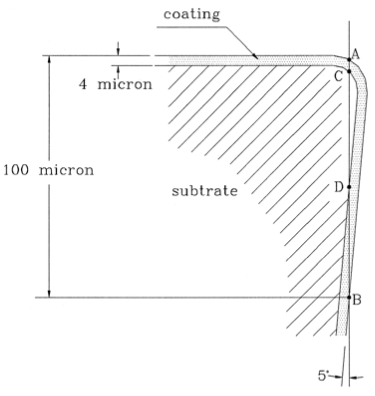
\includegraphics[scale=0.5]{fig/algemeen/plaatjes/Figuren/Insert_construction.png}
	\caption{Construction of the Tool insert with coating. Figure from \citep{Gu1999}}
	\label{fig:alg:insertConstruction}
	\end{figure}
	
	\begin{figure}[hbtp]
	\centering
	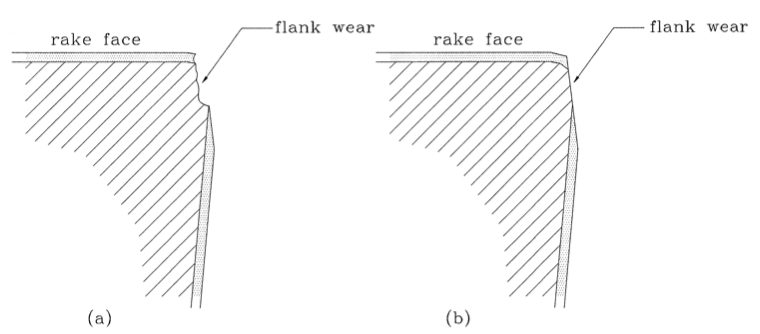
\includegraphics[scale=0.4]{fig/algemeen/plaatjes/Figuren/wear_types.png}
	\caption{Two wear types: (a) Step between substrate and coating. (b) flat wear not perpendicular to the rake face Figure from \citep{Gu1999}}
	\label{fig:gen:insertwears}
	\end{figure}

			
\subsection{Surface of the insert}
	WC typically has a grain size of 0.5 to 2 $\mu$m which is bonded with cobalt that acts as cement between the WC grains. This declares the name of cemented carbides.
			
			
 The next paper is good to get an overview of the light reflection seen in different types of materials and even multi layeres tools.
	article: New color from multilayer coating applied machining tools based on tungsten carbide insert
	J. C. Caicedo1
	\cite{Caicedo2019} Researched the reflectance of coating layers on tool inserts. Here is described that the best reflection occurs at the highest wavelength. This translates to the visible color red and will mean that the reflection should be the highest when the lighting is on the top of the spectrum of the camera lens. 

The material is best cut with a laser at wavelengths 1030nm and 515nm. This is proved in: 
	article: Fundamental investigations of ultrashort pulsed laser ablation on stainless steel and cemented tungsten carbide
	is the good removal also a good reflector?
		
\section{Vision algorithms}
	In this section different vision algorithms will be discussed. 
	
	\subsection{Frameworks}
	- this section may be deleted
	
		There are many frameworks to perform computer vision tasks and make it as easy as possible for the user to get a lot done in a short amount of time. In what follows the different frameworks are listed and shortly documented. \cite{basnet2019towards} provides an overview of different deep learning frameworks. The frameworks used in this thesis are:
		\begin{itemize}
		\item Fast.ai  \citep{fastai} 
		\item Keras \citep{keras} 
		\item PyTorch \citep{pytorch} 
		\end{itemize}
		
		Fast.ai provides a very high level programming experience designed to make deep learning very easy. We found this to be too high level which would affect the customizability of the algorithms.
		Keras is also a high level framework which works with very little programming which is designed for experimenting. 
		PyTorch leaves a little more room for customization. This is the reason PyTorch was used for this thesis. 
		
	\subsection{Architectures for set-up verification}
		Starting from a very small dataset for the creation of a vision set-up, it is nessecary to choose some relevant deep learning network architectures to obtain results which can be compared for different setups. 
		The dataset consists of a little less than 300 images. This constraints the choice of architectures to the ones with very little training parameters since there are not much input images to which the parameters can be trained. In the next sections are some well-known architectures that are used for this determination.
		
		First there must be found an algorithm that can quickly confirm whether a setup is good or not. This will be done by taking pictures from different camera positions with the same lighting. After this the images go trough a simple model and the output is verified with a test set. 
		
		The first algorithm will be Resnet 18 since this is known to to perform well with less parameters and deeper architecture. 
		\cite{Khan2020} extensively describes most available CNN architectures a few of them are used and repeated underneath for a better understanding of the architectures.
		
		\subsubsection{Resnet18}
			First define what Resnet \cite{He2016} means than dig deeper into the Resnet18 architecture.
			
			Resnet is a deep residual neural network that can reach deeper networks without affecting the complexity of the network. What means the amount of parameters or the complexity of the training will not increase much when extra layers are added to the model. 
			The depth of the network plays an important role in the performance. 
			
			Figure \ref{fig:vis:resnetBlock} gives an overview of the important building block which lead to the success of Resnet.  Rather than just stacking layers on top of each other, they provide shortcut connections that skip one or more layers. These shortcut connections perform identity mapping where the outputs are added to the outputs of the stacked layers. This doesn't add extra complexity to the model but allows for more layers to be stacked on top of each other.
			
			\begin{figure}[hbtp]
			\centering
			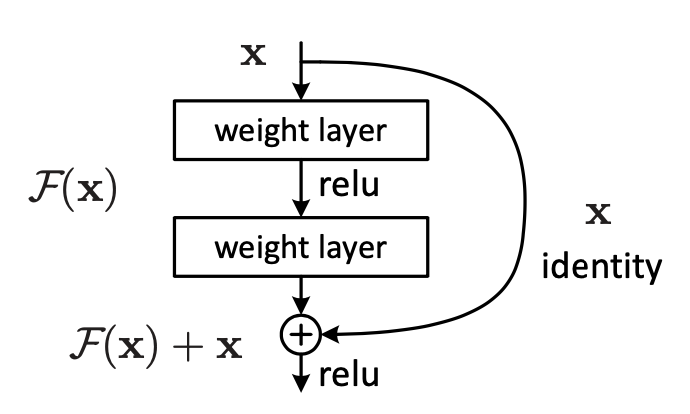
\includegraphics[scale=0.8]{fig/Research/Vision_Algorithm/algorithms/Resnet/resnet_block.png}
			\caption{a building block for Resnet architecture}
			\label{fig:vis:resnetBlock}
			\end{figure}
			
			Figure \ref{fig:vis:resnet18summary} displays a summary of all blocks in the network architecture of Resnet 18. The arrows represent shortcut connections over a few layers. The blocks represent a 3x3 convolution layer where a 3 by 3 grid goes over the previous output and calculates the product with a weight matrix which is updated during training. These calculations provide a new input for the next layer.  The total parameter count for this architecture is 11 million. This seems quite a lot but is actually not much. This will later be compared with other network architectures.
			
			\begin{figure}[hbtp]
			\centering
			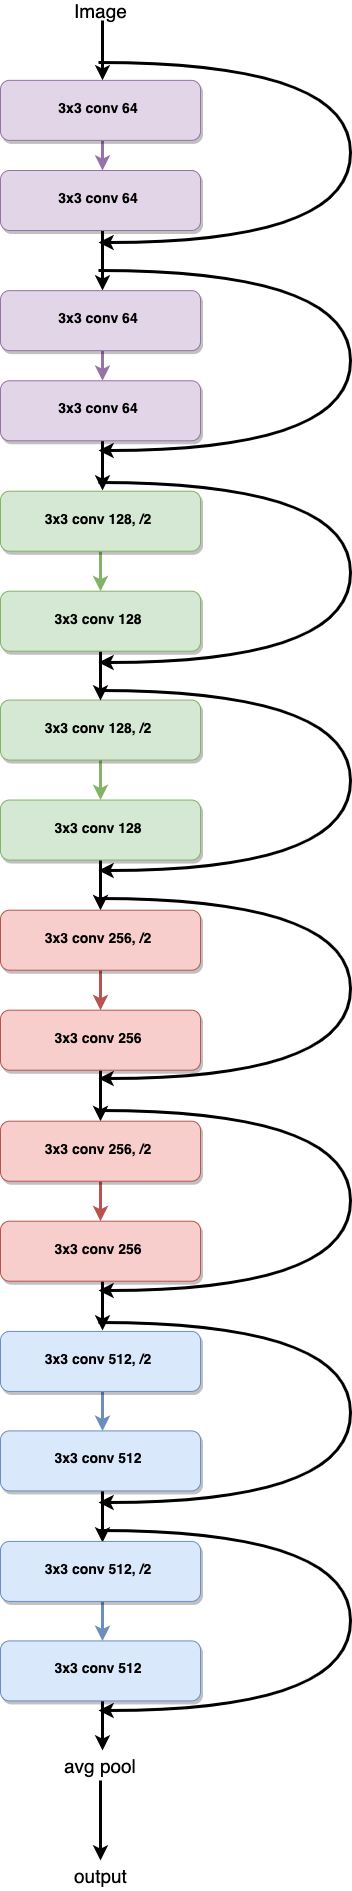
\includegraphics[width=\textwidth, angle=90]{fig/Research/Vision_Algorithm/algorithms/Resnet/Resnet18Diagram.png}
			\caption{Summary of Resnet 18 architecture}
			\label{fig:vis:resnet18summary}
			\end{figure}
			
		
		\subsubsection{VGG11\_bn}
		VGG is a network architecture found by \cite{Simonyan2015} it was designed to get better results at the classification task and does this by using a deeper structure with smaller convolution filters. The original architecture was designed for large scale image classification tasks but will be used for a small dataset in this thesis where VGG is used with 11 layers instead of the original 19 layered architecture.
		
		Batch normalization
		
		\subsubsection{Alexnet}
		Alexnet by \cite{Krizhevsky2017} was one of the first to implement deeper structures in the before known CNN architectures. The implementation of deeper network led to over fitting which was countered with including dropout in the fully connected layers. This makes the model more stable even with more layers. In the time Graphics processing units (GPU's) where not as developed as today so the initial architecture consisted of two parallel paths which could run on two separate GPU's. 
		
		
		
		With 60 million parameters this is more complex as the Resnet 18 architecture 
		
		\subsubsection{Densenet 121}
		
		
		\subsubsection{Squeezenet}
		ToDo

	\subsection{Overview of important numbers}
Parameters and depth for all architectures
	\begin{table}[h!]
\centering
\begin{tabular}{c | c c}
			Model name		& parameters 		& depth (layers) \\ \hline
			Resnet 18			&	11.7 million			&	18 				\\
			VGG11\_bn			&	123.6 million			& 11					\\
			Alexnet				&	61.1 million			& 8					\\
			Densenet 121	&	7.9 million			& 121				\\
			Squeezenet		&	1.2 million			& 10
\end{tabular}
\centering
\caption{Parameters and depth in layers for every model accuracy}
\label{tab:lit:ov:paramdepth}
\end{table}


\subsection{Other architectures for small datasets}

In this section other architectures are explored which received good results on very small image datasets.
The next data input structure is made:

	\begin{itemize}
	\item 20\% train images
	\item 10\% validation images
	\item 10\% test images
	\end{itemize}


These images will go through different algorithms multiple times and the outputs are verified for every different algorithm.

	Very little datasets are available for this problem so all data used in this thesis will be self created. For this reason there are very few images to train and test algorithms on. In what follows are some interesting network architectures given for small dataset image classification. These can later be adjusted to perform image regression tasks.
	
	A first architecture is proposed by \cite{Chandrarathne2019}. They compare training a five layered neural network from scratch and with transfer learning on the imagenet dataset. The findings where that transfer learning could increase the testing accuracy by 10\% on small datasets.
	
	\cite{Xu2019} proposes a so called SDD-CNN what stands for small data driven convolution neural network. This was used for the inspection of roller bearings. A preprocessing method called label dilation is used for dataset imbalance because there is a big imbalance in amount of positive and negative examples. This label dilation method generates random classes where the amount of items per class equals the amount of items in the biggest class. For the roller bearings there are 300 samples per class. After preprocessing the images are augmented to extend the dataset in a controlled way using semi-supervised data augmentation. This process is done by cropping the worn area of the bearing rather than center cropping. Than four networks are trained with the received data. These networks are: 
	\begin{enumerate}
	\item Squeezener v1.1
	\item Inception v3
	\item VGG-16 
	\item ResNet-18
	\end{enumerate}

The findings of the research are that inception v3 performed best for this small dataset when used with transfer learning.


			